%!TEX program = xelatex
\documentclass[dvipsnames, svgnames,a4paper,11pt]{article}
% ----------------------------------------------------- 
%	加边框的命令
%	参考:https://tex.stackexchange.com/questions/531559/how-to-add-the-page-border-for-first-two-pages-in-latex
\usepackage{tikz}
\usetikzlibrary{calc}
\usepackage{eso-pic}
\AddToShipoutPictureBG{%
\begin{tikzpicture}[overlay,remember picture]
\draw[line width=0.6pt] % 边框粗细
    ($ (current page.north west) + (0.6cm,-0.6cm) $)
    rectangle
    ($ (current page.south east) + (-0.6cm,0.6cm) $); % 边框位置
\end{tikzpicture}}


\usepackage{xcolor}
\definecolor{c1}{HTML}{070F94} % 目录颜色 原版为2752C9 紫灰色535AAA 蓝紫色0B0DB7 深蓝色070F94 湖绿色219394 松石灰绿086173
\definecolor{c2}{HTML}{E20129} % 引用颜色 原版\definecolor{c2}{RGB}{190,20,83} 橙色F24729

\usepackage{ctex}
\usepackage[top=28mm,bottom=28mm,left=15mm,right=15mm]{geometry}
\usepackage{hyperref} 
\hypersetup{
	colorlinks,
	linktoc = section, % 超链接位置,选项有section, page, all
	linkcolor = c1, % linkcolor 目录颜色
	citecolor = c1  % citecolor 引用颜色
}
\usepackage{amsmath,enumerate,multirow,float}
\usepackage{tabularx}
\usepackage{tabu}
\usepackage{subfig}
\usepackage{fancyhdr}
\usepackage{graphicx}
\usepackage{wrapfig}  
\usepackage{physics}
\usepackage{appendix}
\usepackage{amsfonts}

%
\usepackage{tcolorbox}
\tcbuselibrary{skins,breakable}
\newtcolorbox{tbox}[2][]{
    colframe=black!70!,
    breakable,
    enhanced,
	boxrule =0.5pt,
    title = {#2},
    fonttitle = \large\kaishu\bfseries,
	drop fuzzy shadow,
    #1
}
\newtcolorbox[auto counter,number within=section]{question}[1][]{
  top=2pt,bottom=2pt,arc=1mm,
  boxrule=0.5pt,
%   frame hidden,
  breakable,
  enhanced, %跨页后不会显示下边框
  coltitle=c1!80!gray,
  colframe=c1,
  colback=c1!3!white,
  drop fuzzy shadow,
  title={思考题~\thetcbcounter:\quad},
  fonttitle=\bfseries,
  attach title to upper,
  #1
}

% ---------------------------------------------------------------------
%	利用cleveref改变引用格式,\cref是引用命令
\usepackage{cleveref}
\crefformat{figure}{#2{\textcolor{c2}{Figure #1}}#3} % 图片的引用格式
\crefformat{equation}{#2{(\textcolor{c2}{#1})}#3} % 公式的引用格式
\crefformat{table}{#2{\textcolor{c2}{Table #1}}#3} % 表格的引用格式


% ---------------------------------------------------------------------
%	页眉页脚设置
\fancypagestyle{plain}{\pagestyle{fancy}}
\pagestyle{fancy}
\lhead{\kaishu 中山大学物理与天文学院基础物理实验\uppercase\expandafter{\romannumeral2}} % 左边页眉,学院 + 课程
\rhead{\kaishu 实验报告By黄罗琳} % 右边页眉,实验报告标题
\cfoot{\thepage} % 页脚,中间添加页码


% ---------------------------------------------------------------------
%	对目录、章节标题的设置
\renewcommand{\contentsname}{\centerline{\huge 目录}}
\usepackage{titlesec}
\usepackage{titletoc}
% \titleformat{章节}[形状]{格式}{标题序号}{序号与标题间距}{标题前命令}[标题后命令]
\titleformat{\section}{\centering\LARGE\songti}{}{1em}{}

% ---------------------------------------------------------------------
%   listing代码环境设置
\usepackage{listings}
\lstloadlanguages{python}
\lstdefinestyle{pythonstyle}{
backgroundcolor=\color{gray!5},
language=python,
frameround=tftt,
frame=shadowbox, 
keepspaces=true,
breaklines,
columns=spaceflexible,                   
basicstyle=\ttfamily\small, % 基本文本设置,字体为teletype,大小为scriptsize
keywordstyle=[1]\color{c1}\bfseries, 
keywordstyle=[2]\color{Red!70!black},   
stringstyle=\color{Purple},       
showstringspaces=false,
commentstyle=\ttfamily\scriptsize\color{green!40!black},%注释文本设置,字体为sf,大小为smaller
tabsize=2,
morekeywords={as},
morekeywords=[2]{np, plt, sp},
numbers=left, % 代码行数
numberstyle=\it\tiny\color{gray}, % 代码行数的数字字体设置
stepnumber=1,
rulesepcolor=\color{gray!30!white}
}




% ---------------------------------------------------------------------
%	其他设置
\def\degree{${}^{\circ}$} % 角度
\graphicspath{{./images/}} % 插入图片的相对路径
\allowdisplaybreaks[4]  %允许公式跨页 
\usepackage{lipsum}
\usepackage{adjustbox}
\usepackage{subcaption}

%\usepackage{mathrsfs} % 字体
%\captionsetup[figure]{name=Figure} % 图片形式
%\captionsetup[table]{name=Table} % 表格形式
\begin{document}
	
	% 实验报告封面	
	% 顶栏
	\begin{table}
		\renewcommand\arraystretch{1.7}
		\begin{tabularx}{\textwidth}{
				|X|X|X|X
				|X|X|X|X|}
			\hline
			\multicolumn{2}{|c|}{预习报告}&\multicolumn{2}{|c|}{实验记录}&\multicolumn{2}{|c|}{分析讨论}&\multicolumn{2}{|c|}{总成绩}\\
			\hline
			\LARGE25 & & \LARGE25 & & \LARGE30 & & \LARGE80 & \\
			\hline
		\end{tabularx}
	\end{table}
	% ---
	
	% 信息栏
	\begin{table}
		\renewcommand\arraystretch{1.7}
		\begin{tabularx}{\textwidth}{|X|X|X|X|}
			\hline
			年级、专业: & 2022级 物理学 &组号:教学班1 & \\
			\hline
			姓名: & 黄罗琳   & 学号: &22344001   \\
			\hline
			实验时间: & 2024/3/21 & 教师签名: & \\
			\hline
		\end{tabularx}
	\end{table}
	% ---
	
	% 大标题
	\begin{center}
		\LARGE CD1\quad 光学像差测量与分析
	\end{center}
	% ---
	
	% 注意事项
	
	% 基本
	\textbf{【实验报告注意事项】}
	\begin{enumerate}
		\item 实验报告由两部分组成:
		\begin{enumerate}
			\item 预习报告:课前认真研读实验讲义,弄清实验原理;实验所需的仪器设备、用具及其使用、完成课前预习思考题;了解实验需要测量的物理量,并根据要求提前准备实验记录表格(可以参考实验报告模板,可以打印)。(30分)
			\item 实验记录与分析:认真、客观记录实验条件、实验过程中的现象以及数据。实验记录请用珠笔或者钢笔书写并签名(用铅笔记录的被认为无效)。保持原始记录,包括写错删除部分,如因误记需要修改记录,必须按规范修改。(不得手记的值输入到电脑打印);离开前请实验教师检查记录并签名。(50分)
		\end{enumerate}
		
		\item\textcolor{red}{ 本实验报告可提前打印出来,当场记录分析完成交给带实验的老师,课后无需再提交。若当场完成不了,则请课后完成,再扫描并通过seelight提交。}\\
		\textcolor{red}{\colorbox{yellow}{注意:本文档已留出填写空间,若填写空间不够的话请提前规划留白,做到报告的美观)}}
		\item 注意事项:
		\begin{enumerate}
			\item 实验中避免激光器伤到眼睛
			\item 避免用手直接接触镜片的光学面
			\item 安装镜片时需在光学平台上尽量靠近台面的高度操作,以免失手跌落摔碎镜片
			\item 实验平台配件所用固定螺钉需拧紧,以免镜架晃动;但不可过紧,以免损坏
			\item 实验前需按仪器清单检查光学元件是否齐全,实验结束后按照顺序放回元件盒
		\end{enumerate}
		
		\end{enumerate}
	
	
	% 目录
	\clearpage
	\tableofcontents
	\clearpage
	% ---
	
	
	
	% 预习报告	
	
	% 小标题
	\setcounter{section}{0}
	\section{CD1\quad 光学像差测量与分析 \heiti 预习报告}
	% ---
	
	% 实验目的
	\subsection{实验目的}
	\begin{enumerate}
		\item 了解七种几何像差产生的原理、基本规律;
		\item 了解各种像差对光学成像质量的影响;
		\item 掌握慧差、色差产生的原理及其测量表征;
		\item 掌握光学系统的基本调试方法;
	\end{enumerate}
	% ---
	
	% 仪器用具
	\subsection{仪器用具}
	\begin{table}[htbp]
		\centering
		\begin{tabular}{|c|c|c|c|}
			\hline
			
			\textbf{产品编号} & \textbf{产品名称} & \textbf{规格}          & \textbf{数量} \\ \hline
			1                & 激光光源           & λ=632.6nm            & 1            \\ \hline
			2                & 激光器夹持器       & 3维调整               & 1            \\ \hline
			3                & 显微物镜           & 10×/0.25             & 1            \\ \hline
			4                & 针孔               & Ø100um或Ø50um       & 1            \\ \hline
			5                & 五维调整机构       & 装配显微物镜和针孔用 & 1            \\ \hline
			6                & 衰减片1            & 0.0001(衰减系数)  & 1            \\ \hline
			7                & 衰减片2            & 0.01(衰减系数)     & 1            \\ \hline
			8                & 双凸透镜1          & 焦距f=300mm         & 1            \\ \hline
			9                & 平凸透镜2          & 焦距f=100mm         & 1            \\ \hline
			10               & 平凸透镜3          & 焦距f=150mm         & 1            \\ \hline
			11               & 白屏               & SZ-13,一面白屏,一面带坐标纸 & 1 \\ \hline
			12               & 成像相机           & 大恒的MER-130-30UM或元启智能的REV-13AMU2C & 1 \\ \hline
			13               & 数据线             & 图像采集数据线       & 1            \\ \hline
			14               & 计算机             & 台式或笔记本,安装有成像相机图像采集软件 & 1 \\ \hline
			15               & 光学导轨           & 长度1米,带刻度      & 1            \\ \hline
			16               & 二维平移台         & 行程>10mm            & 4            \\ \hline
			17               & 平移滑块           &                      & 8            \\ \hline
			18               & 支杆               & 50mm长和75mm长       & 3+5          \\ \hline
			19               & 磁性表座           &                      & 4            \\ \hline
			20               & 旋转调整台         & 可调角度>±5°        & 1            \\ \hline
			21               & 白光灯             & GY-6型,亮度可调,即溴钨灯 & 1     \\ \hline
			22               & 滤光片1            & 透光波长:435nm       & 1            \\ \hline
			23               & 滤光片2            & 透光波长:630nm       & 1            \\ \hline
			\end{tabular}
			\end{table}
			
	% ---
	
	% 原理概述
	\subsection{原理概述}
	
当光线穿过透镜或其他光学元件时,由于光的波长不同,其在介质中的折射率也会有所不同。这导致了色差和慧差这两种光学现象的产生。

\begin{enumerate}
    \item \textbf{色差(Chromatic Aberration)}:
    
    色差主要由两个因素引起:球面色差和色散色差。
    
    \begin{itemize}
        \item \textbf{球面色差}:当光线通过球面透镜或球面镜面时,由于球面形状的限制,不同部位的光线折射程度不同,导致不同颜色的光聚焦于不同位置。具体而言,透镜的中心部位对光线的折射程度比较大,而边缘部位则较小。因此,蓝色光会被更多地折射,使其焦点位置比红色光更接近透镜,从而导致不同波长的光聚焦位置不同。
        
        \item \textbf{色散色差}:不同波长的光在透明介质中传播时,其折射率会有所不同,即介质对不同波长的光有不同的折射率。因此,当白光通过透镜或透明介质时,不同波长的光会以不同的角度折射,导致不同颜色的光被分散开来,形成彩色边缘或色彩偏移。
    \end{itemize}
    
    解决色差问题的方法包括使用复合透镜、消色差镜片、非球面透镜等,以及在设计光学系统时考虑到色差校正的需求。
    
    \item \textbf{慧差(Spherical Aberration)}:
    
    慧差是由于球面透镜或球面镜面的几何形状限制而引起的。当光线通过球面透镜或球面镜面时,焦点位置不再是一个确定的点,而是在一定的范围内分散,使成像产生模糊、失真或虚影。
    
    慧差的解决方法包括使用非球面透镜或透镜组合、添加补偿光学元件等。非球面透镜具有非常复杂的曲率,可以根据需要设计,使光线聚焦到更小的焦点上,从而减小慧差带来的影响,提高成像质量。
    
在光学系统设计中,通常需要综合考虑色差和慧差以及其他光学畸变,以确保获得高质量的成像效果。这涉及到对光学元件的选择、设计和优化,以满足特定应用的要求。

\end{enumerate}



	
	
	
	% 实验前思考题
	\subsection{实验前思考题}
	
	% 思考题1
	\begin{question}
		慧差与孔径、视场的关系?
	\end{question}
	\begin{enumerate}
		\item \textbf{慧差与孔径、视场的关系}:
		\begin{enumerate}
			\item 慧差与孔径的关系:
		
				随着孔径的增大,慧差的影响会增加。
				较大的孔径会导致更多的光线经过光学元件的边缘部分,而慧差通常是由于边缘部分的光线与中心部分的光线聚焦位置不同而引起的。因此,较大的孔径会加剧慧差的影响。
			
			
			\item 慧差与视场的关系:
			\
				视场的大小也会影响慧差的表现。当视场较大时,光线来自不同方向和角度的目标会聚焦在像平面上不同的位置,这可能会加剧慧差现象。特别是对于较大的视场,由于不同位置的光线需要通过透镜或镜面,而不同位置的光线折射程度可能会有所不同,导致成像的模糊和失真现象更加显著。
			
		\end{enumerate}
	\end{enumerate}
	
	% 思考题2
	\begin{question}
			产生色差原因?列举几种消色差的方法
	\end{question}
	产生色差原因见实验原理。以下是几种消色差的方法:
\begin{enumerate}
    \item 使用复合透镜,由不同玻璃材料制成,以抵消不同波长光线的色散效应。
    \item 使用非球面透镜,具有非球形曲率,可以根据需要设计,减少色差现象。
    \item 使用消色差棱镜,由不同材料制成的棱镜组合,减少色差。
    \item 使用色散补偿镜片,设计用于校正色散,使得不同波长的光线具有相同的光程,减少色差效应。
\end{enumerate}
	% 思考题3
	\begin{question}
		针孔滤波的工作原理
	\end{question}
	针孔滤波器的工作原理基于衍射现象。当光线通过非常小的孔口时,光波会在孔边缘发生衍射,形成一系列明暗相间的环形条纹或衍射图样。\\

针孔滤波器的工作原理主要包括以下几点:
\begin{enumerate}
    \item 衍射效应:光线通过针孔时会发生衍射现象,使光在屏幕上形成衍射图样。
    \item 孔径大小:针孔的直径决定了衍射图样的特征,较小的孔径会产生更多的衍射效应。
    \item 滤波作用:针孔滤波器用于滤波或选择特定波长范围的光,通过选择合适的孔径大小和观察位置实现滤波效果。
    \item 分辨能力:针孔滤波器的分辨能力取决于孔径的大小,较小的孔径具有更好的分辨能力。
\end{enumerate}

因此,针孔滤波器可以根据衍射现象实现光学滤波的目的
	% ---
	
	
	
	% 实验记录	
	\clearpage
	
	% 顶栏
	\begin{table}
		\renewcommand\arraystretch{1.7}
		\centering
		\begin{tabularx}{\textwidth}{|X|X|X|X|}
			\hline
			专业: & 物理学 & 年级: & 2022级 \\
			\hline
			姓名: & 黄罗琳 & 学号: &22344001 \\
			\hline
			室温: & 23℃ & 实验地点: & A522 \\
			\hline
			学生签名:& 
\includegraphics[width=1cm]{签字.jpg} & 评分: &\\
			\hline
			实验时间:& 2024/3/21 & 教师签名:&\\
			\hline
		\end{tabularx}
	\end{table}
	% ---
	
	% 小标题
	\section{CD1 光学像差测量与分析 \quad\heiti 实验记录}
	% ---
	
	% 实验过程记录
	\subsection{实验内容、步骤与结果}
	
	%
	\subsubsection{操作步骤记录}
	
	
	实验光路如图 \ref{位置色差} 所示。实验步骤如下:
	\begin{enumerate}
\item 色差测量实验

	\begin{enumerate}
		\item 按图示光路,先摆放溴钨灯、透镜、白屏,调整透镜4的中心高与光源等高,使光源在透镜4的物方1~2倍焦距处,调整白屏的位置,找到溴钨灯灯丝最清晰的像位置,并记录该位置;
		\item 按图示光路,放置滤光片1,调整白屏的位置,找到溴钨灯丝最清晰的像位置并记录白屏位置;
		\item 更换为滤光片2,再调整白屏的位置,找到这时溴钨灯丝最清晰的像位置并记录白屏位置;
		\item 计算位置色差;判断波长与折射率之间的关系。
	\end{enumerate}
	\begin{figure}[H]
		\centering
		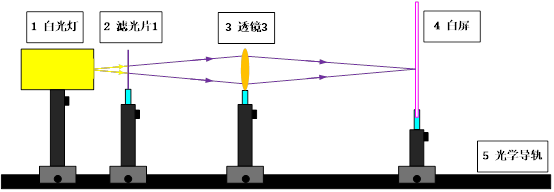
\includegraphics[width=0.8\textwidth]{位置色差.png}
		\caption{位置色差测量光路图}
		\label{位置色差}
	\end{figure}
	\item 光路调试与慧差测量实验\\
	实验光路如图 \ref{慧差}所示。实验步骤如下:
	\begin{enumerate}
		\item 根据图示布局及元器件参数,估计各器件的摆放位置,并做初步的预调整。
		\item 放置激光器,打开光源,安装白屏在滑块上,移动白屏以调整激光器方位和俯仰,使光点位置基本不变;固定白屏,并标记光斑位置。
		\item 安装显微物镜和针孔到五维调整机构上,让激光正入射显微物镜。调整针孔位置,使其位于焦点位置,产生环形衍射光斑。微调五维调整机构,使光斑中心位于标记位置。固定显微物镜和针孔位置。
		\item 安装双凸透镜1,对发散球面波进行准直。调整透镜位置,使光斑与镜面同心,并使针孔位于透镜焦点位置,得到近似平行光。
		\item 安装平凸透镜2(或平凸透镜3),调整位置使入射光斑与镜面同心,并方便后续角度调整。
		\item 安装衰减片1和成像相机。调整相机位置,使其靶面位于平凸透镜2焦点处,采集图像。
		\item 调整旋转调整机构的角度,使平凸透镜2发生偏转,观察并记录焦点图像、焦前图像、焦后图像,并记录偏转角度。选取5个角度点,记录对应的图像,分析慧差随角度变化关系。
		
	\end{enumerate}
	\begin{figure}[H]
		\centering
		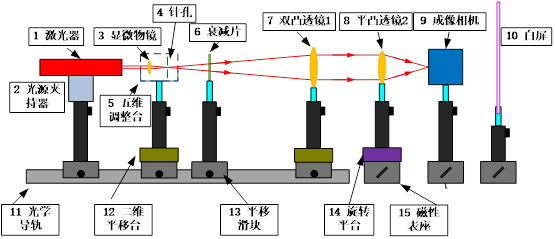
\includegraphics[width=0.8\linewidth]{慧差光路.png}
		\caption{慧差观测光路图}
		\label{慧差}
	\end{figure}
\end{enumerate}
\subsubsection{实验原始数据}

\subsubsection{实验图像汇总}
\begin{figure}[H]
	\begin{minipage}[b]{0.3\linewidth}
	  \centering
	  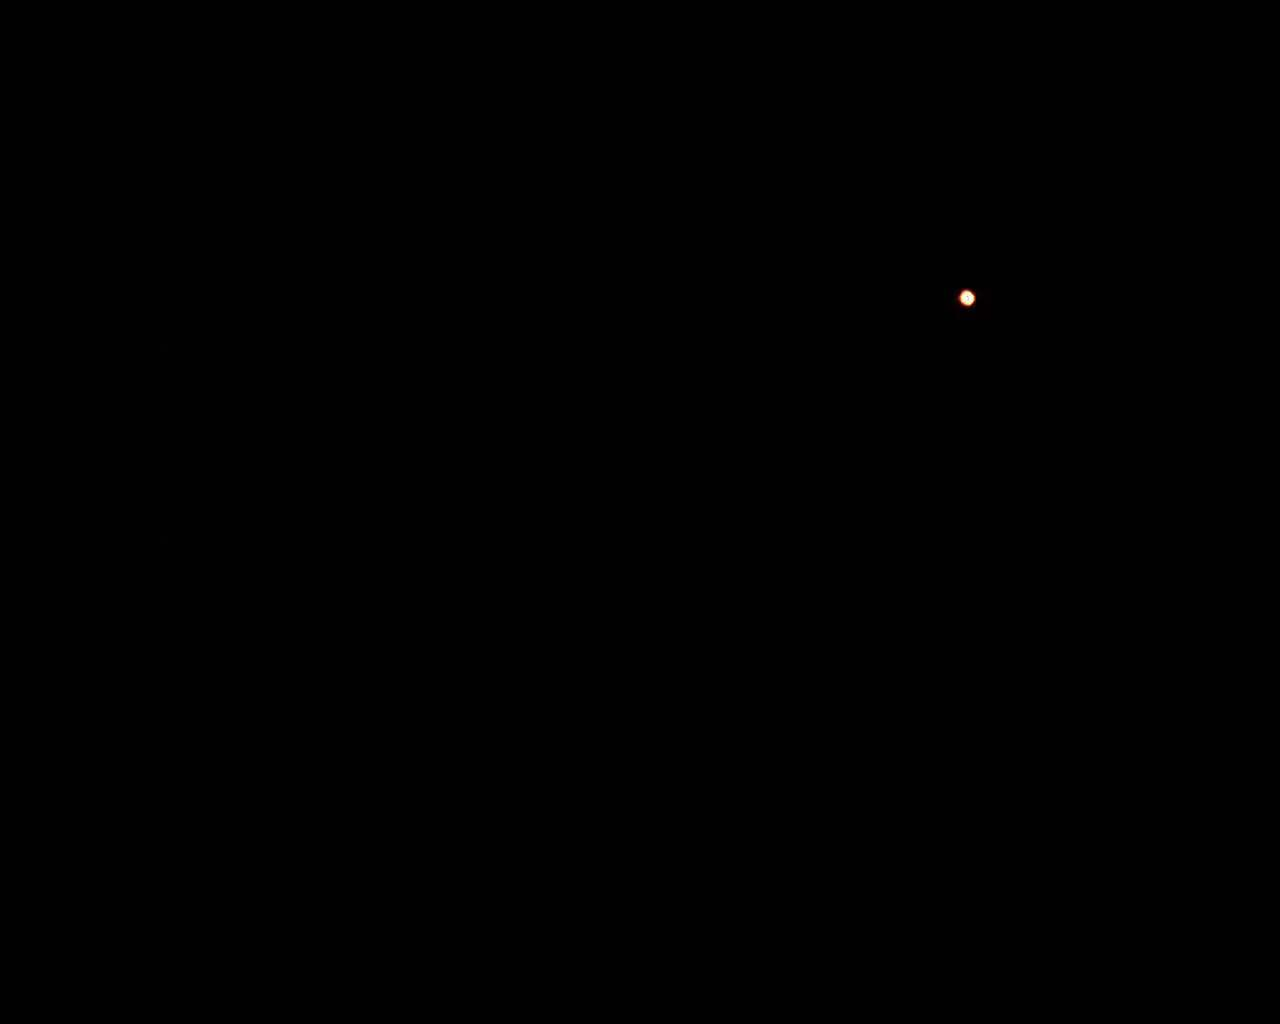
\includegraphics[width=\linewidth]{焦点0.jpg}
	  \caption{焦点图像}
	  \label{fig:sub1}
	\end{minipage}
	\hfill
	\begin{minipage}[b]{0.3\linewidth}
	  \centering
	  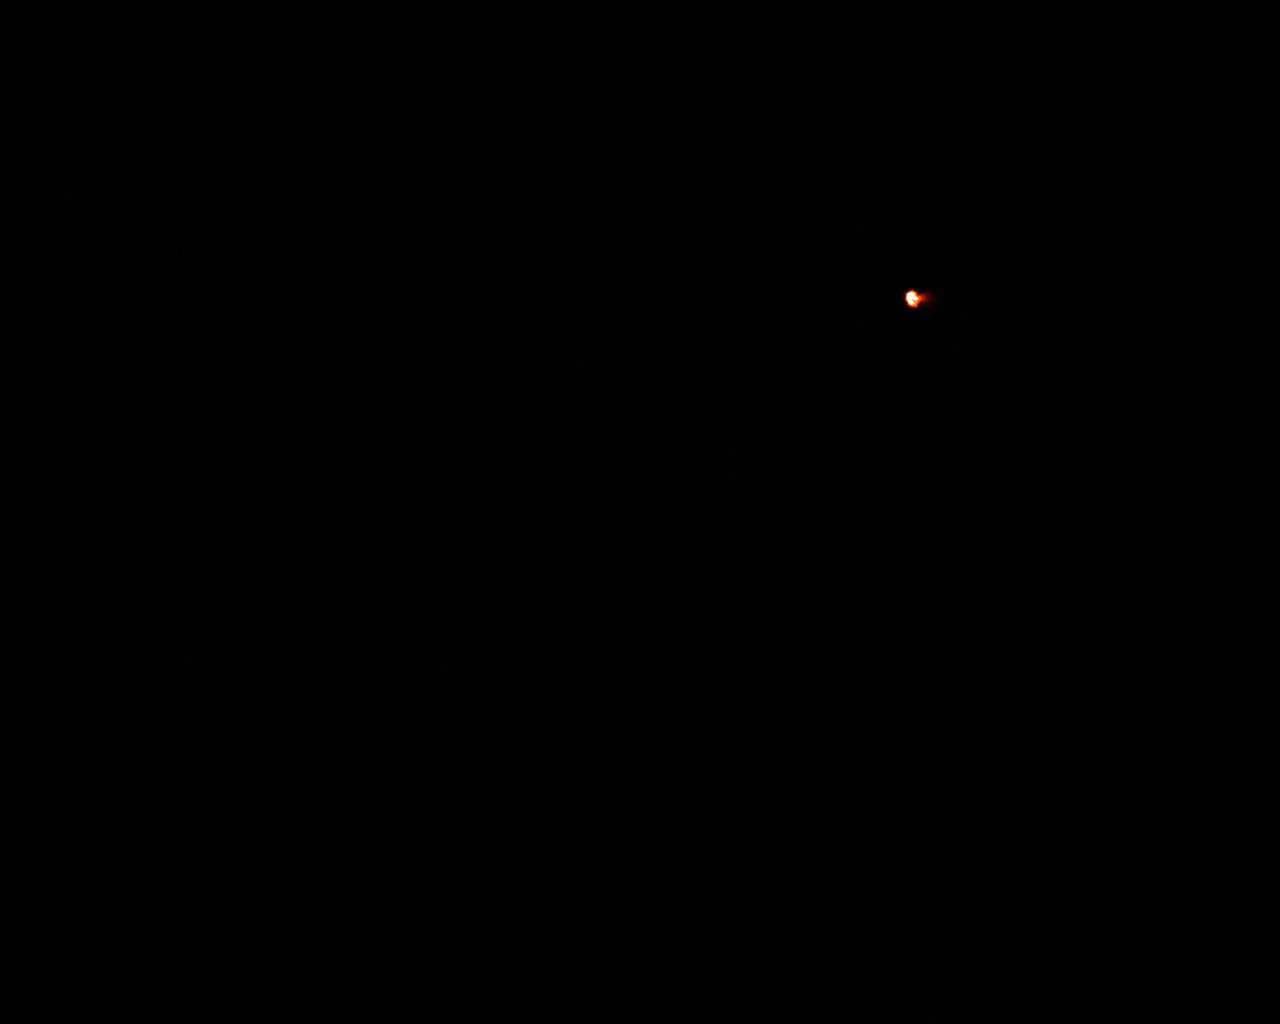
\includegraphics[width=\linewidth]{逆时针5.jpg}
	  \caption{逆时针5°}
	  \label{fig:sub2}
	\end{minipage}
	\hfill
	\begin{minipage}[b]{0.3\linewidth}
	  \centering
	  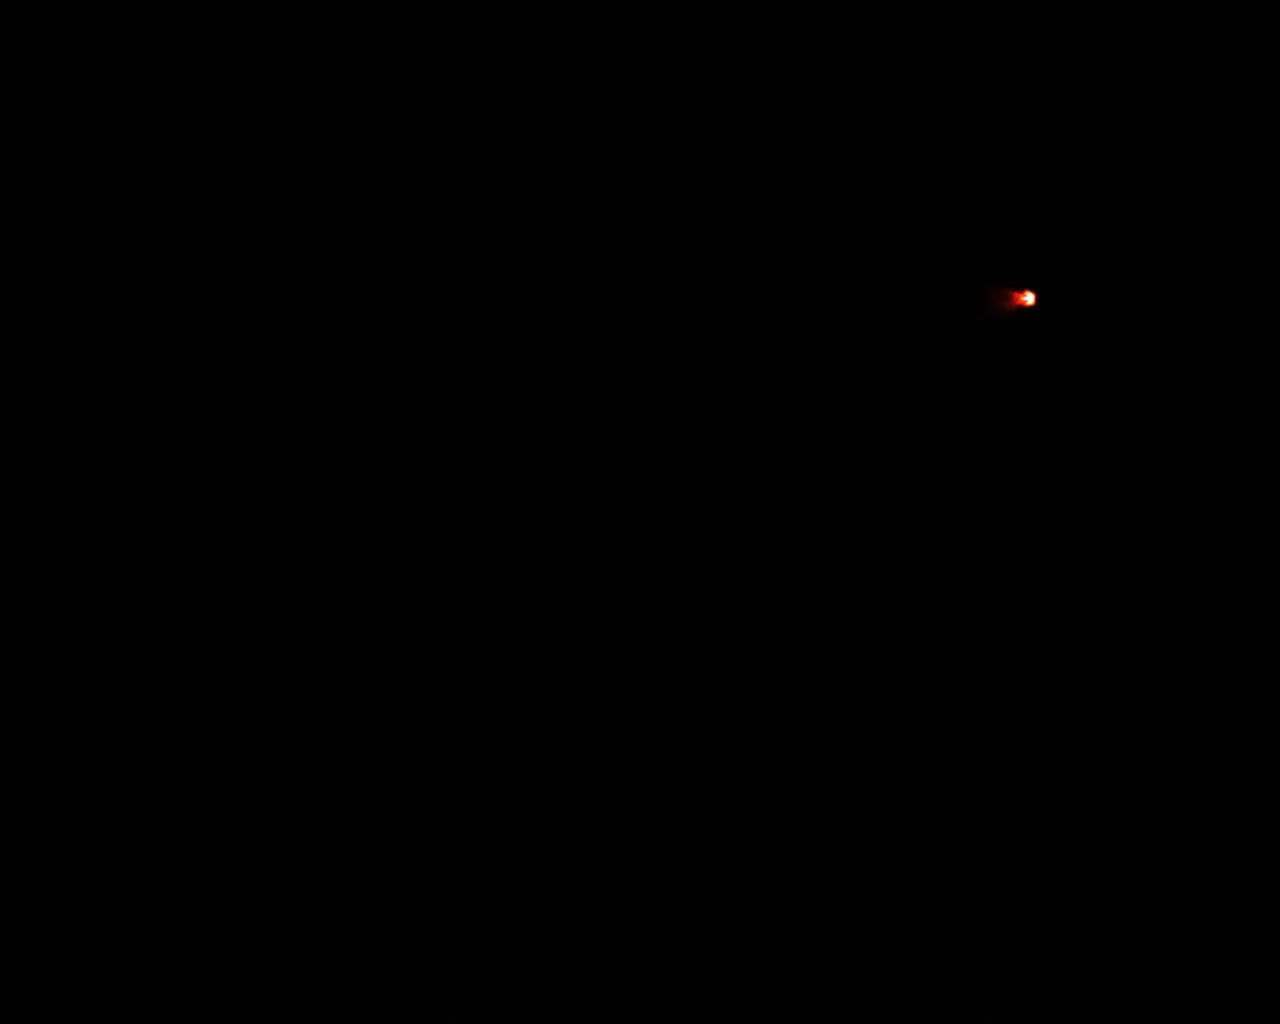
\includegraphics[width=\linewidth]{顺时针5.jpg}
	  \caption{顺时针5°}
	  \label{fig:sub3}
	\end{minipage}
  \end{figure}
  

  \begin{figure}[H]
	\begin{minipage}[b]{0.3\linewidth}
	  \centering
	  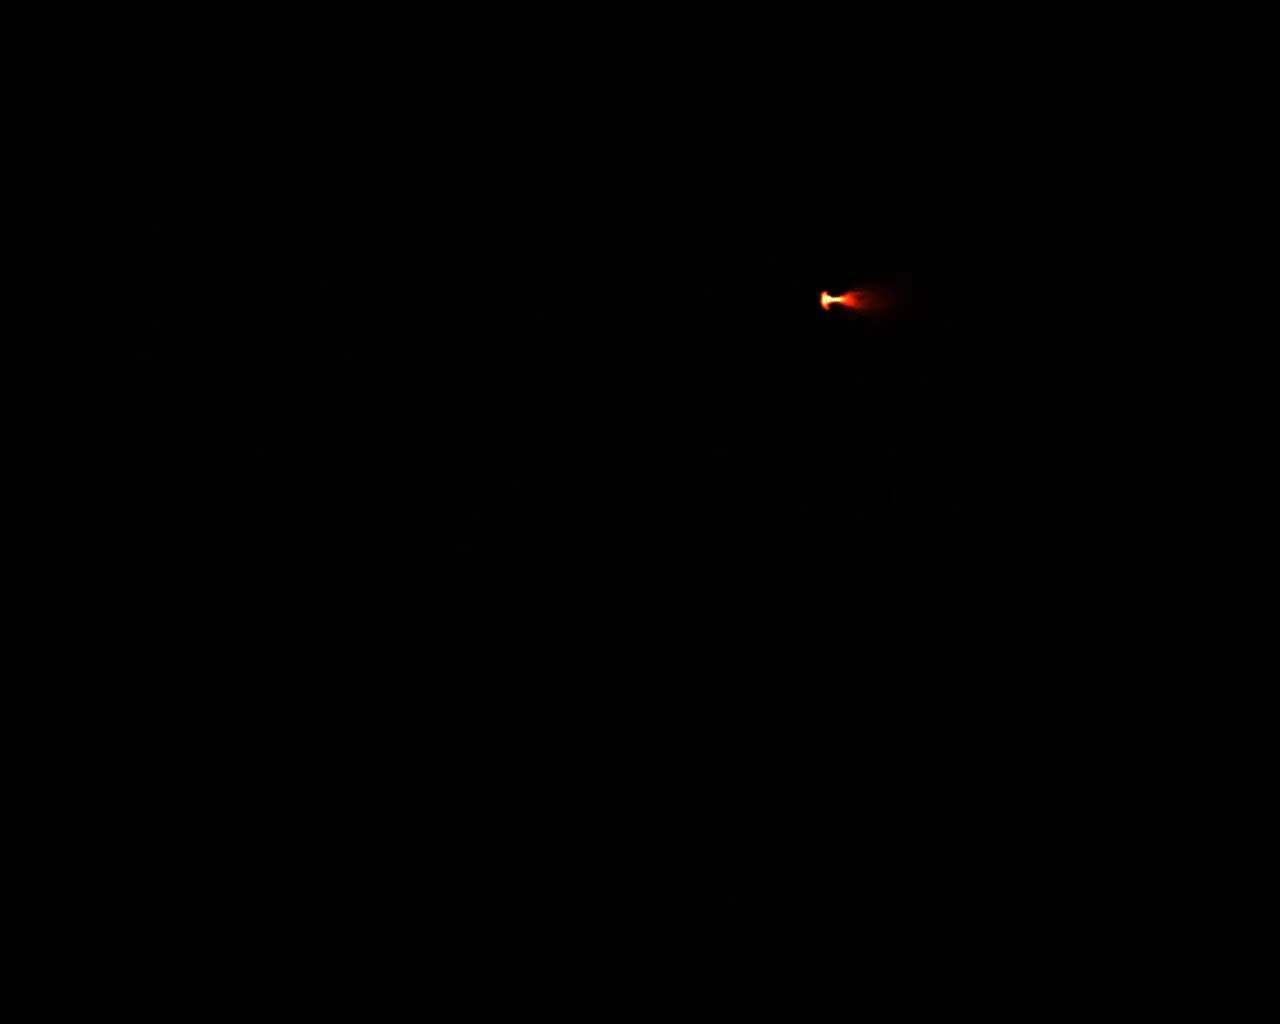
\includegraphics[width=\linewidth]{逆时针10.jpg}
	  \caption{逆时针10°}
	  \label{fig:sub1}
	\end{minipage}
	\hfill
	\begin{minipage}[b]{0.3\linewidth}
	  \centering
	  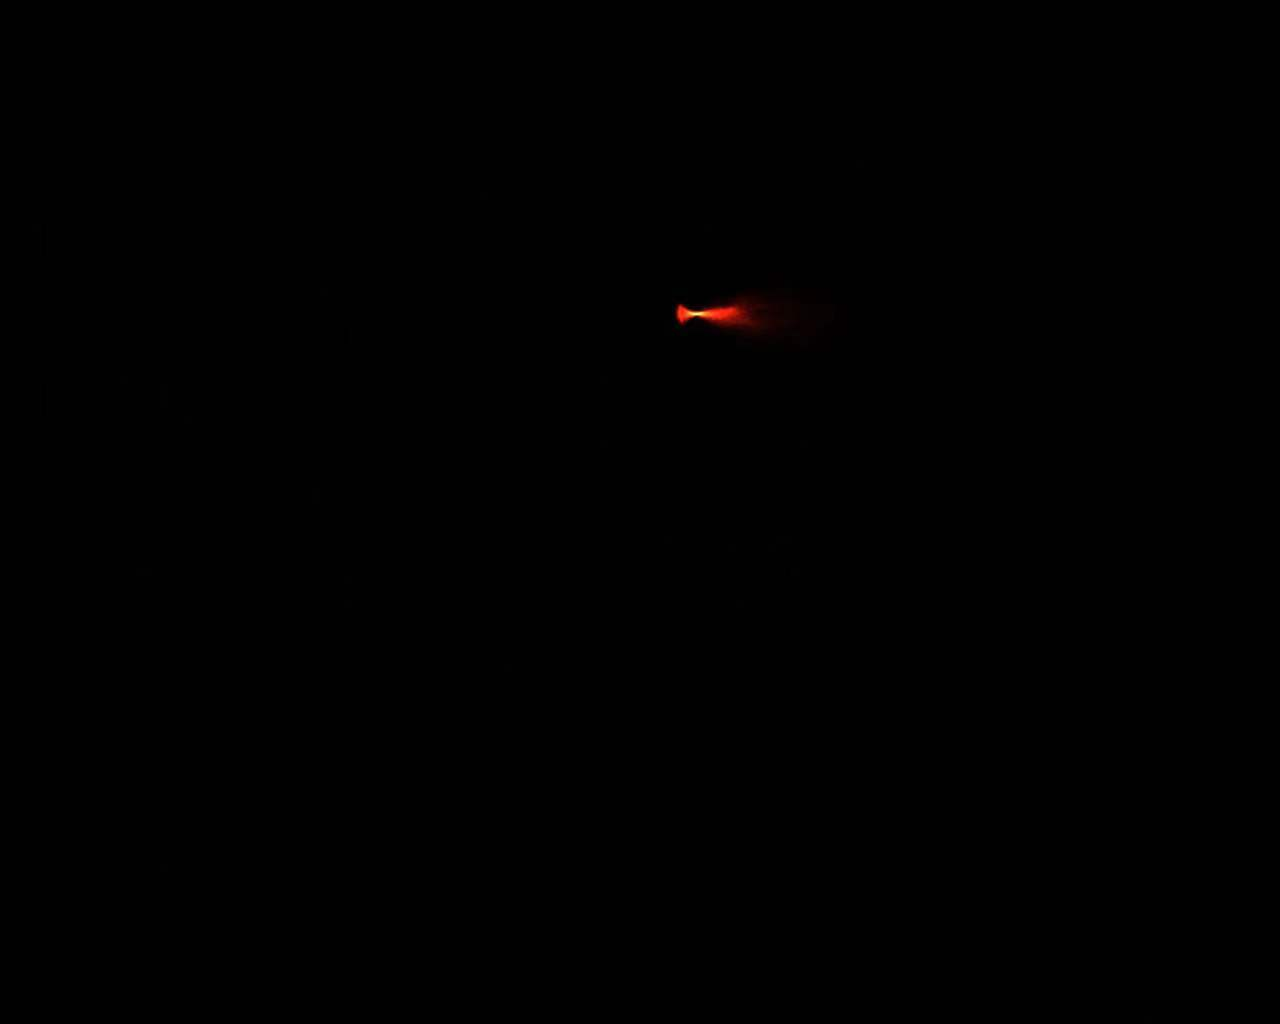
\includegraphics[width=\linewidth]{逆时针15.jpg}
	  \caption{逆时针15°}
	  \label{fig:sub2}
	\end{minipage}
	\hfill
	\begin{minipage}[b]{0.3\linewidth}
	  \centering
	  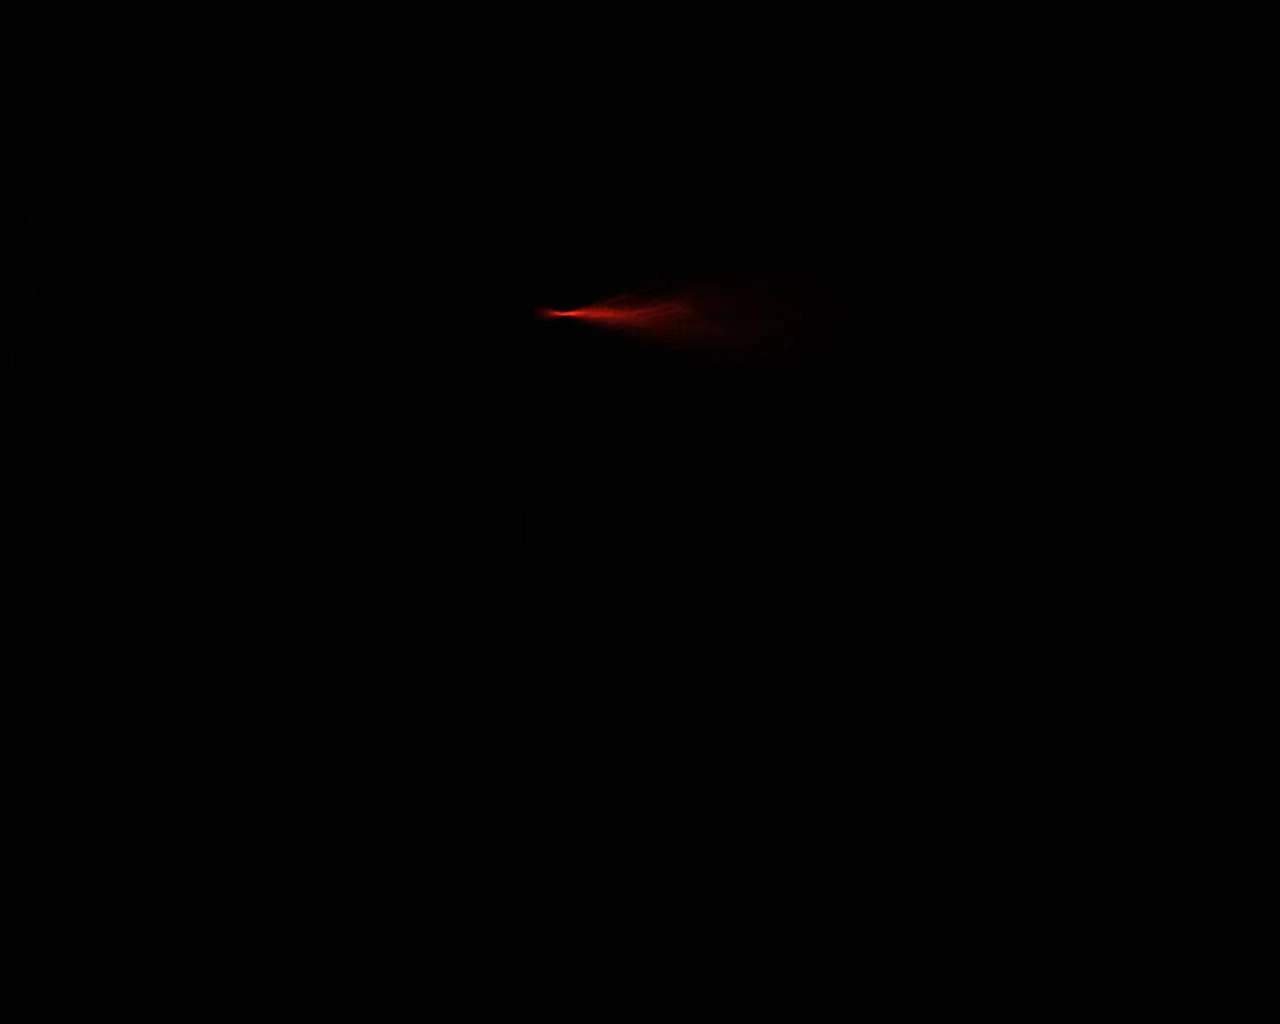
\includegraphics[width=\linewidth]{逆时针20.jpg}
	  \caption{逆时针20°}
	  \label{fig:sub3}
	\end{minipage}
  \end{figure}
  
  \begin{figure}[H]
	\begin{minipage}[b]{0.3\linewidth}
	  \centering
	  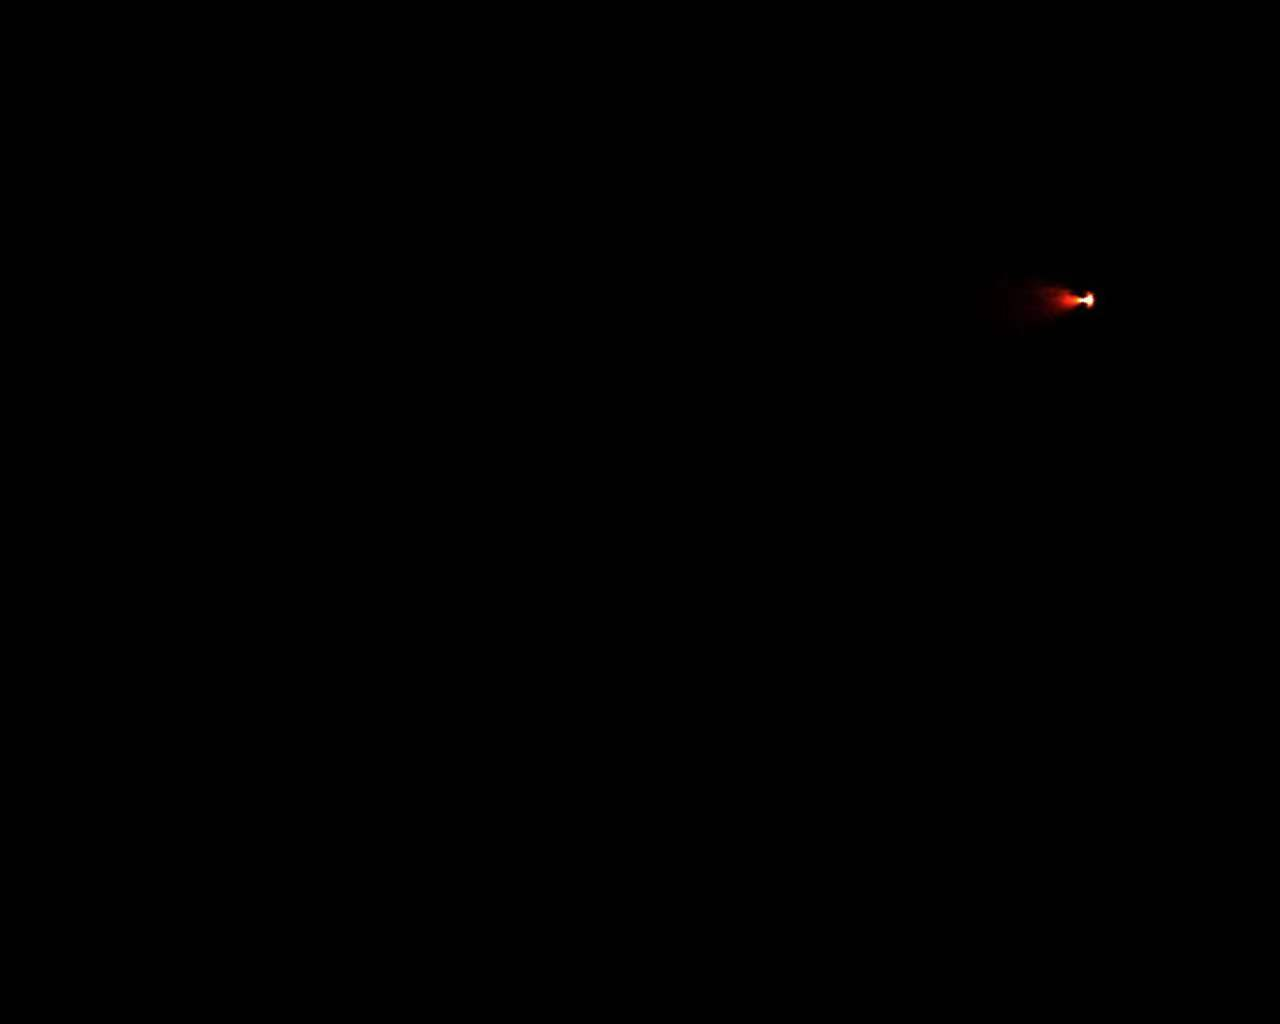
\includegraphics[width=\linewidth]{顺时针10.jpg}
	  \caption{顺时针10}
	\end{minipage}
	\hfill
	\begin{minipage}[b]{0.3\linewidth}
	  \centering
	  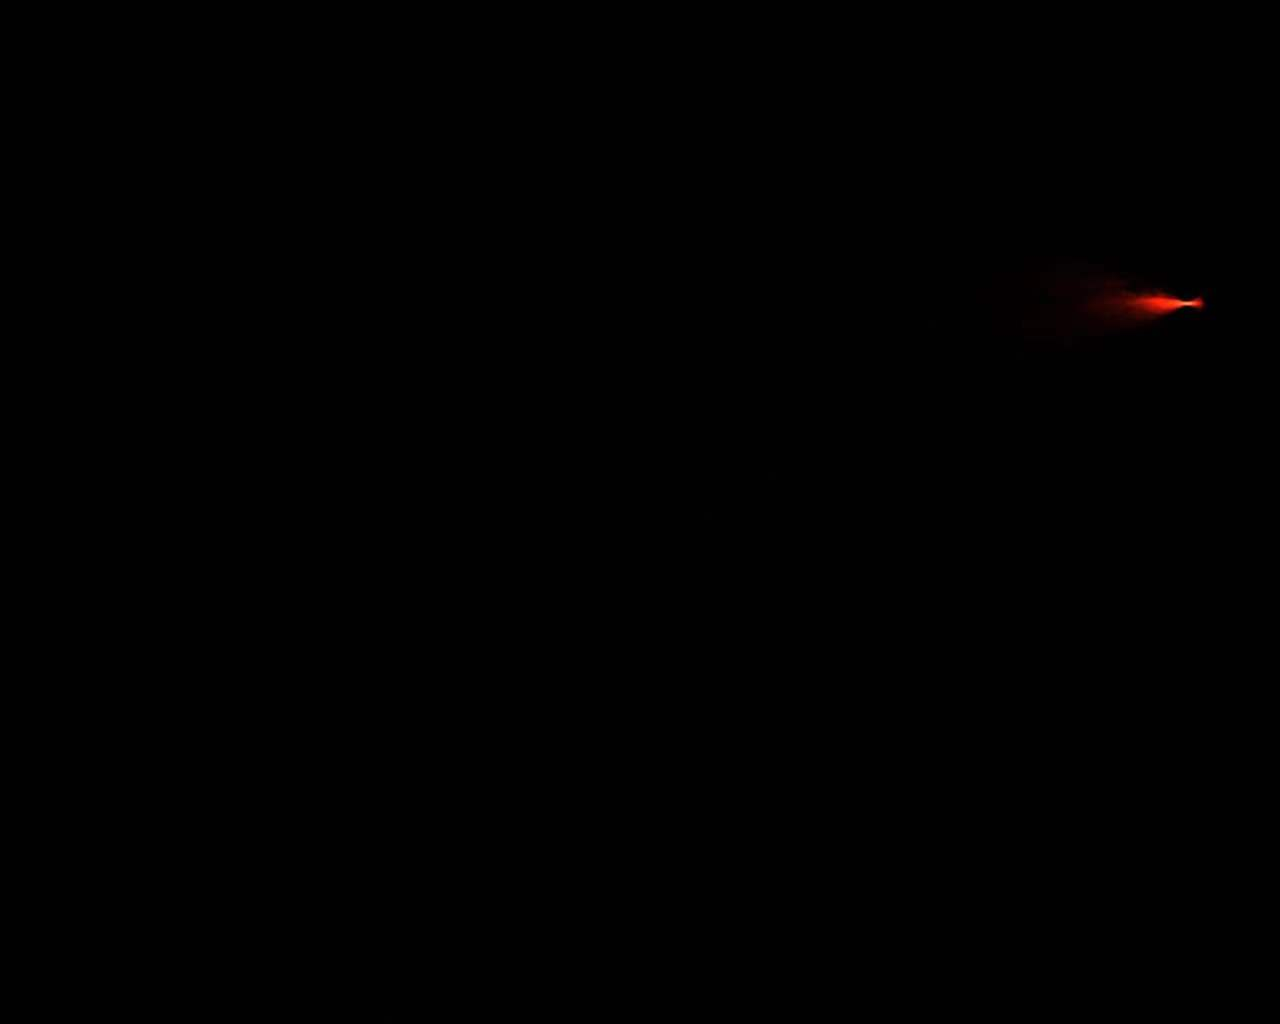
\includegraphics[width=\linewidth]{顺时针15.jpg}
	  \caption{顺时针15}
	\end{minipage}
	\hfill
	\begin{minipage}[b]{0.3\linewidth}
	  \centering
	  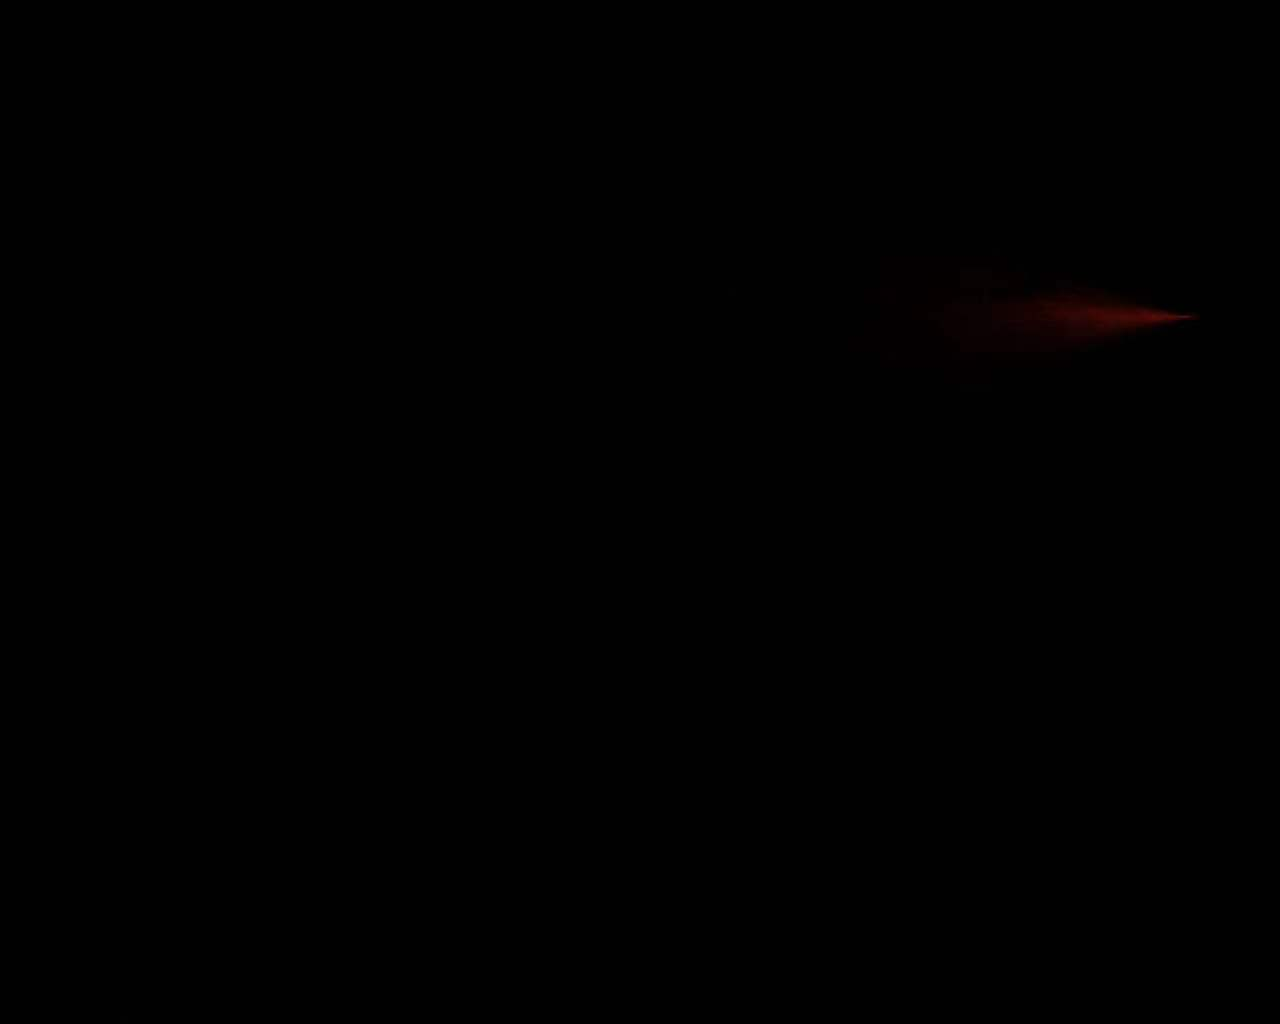
\includegraphics[width=\linewidth]{顺时针20.jpg}
	  \caption{顺时针20}
	\end{minipage}
  \end{figure}


	
	% 问题记录
	\subsection{实验过程遇到问题及解决办法}
	\begin{enumerate}
		\item 首先由于仪器14旋转平台的高度存在最低限度,从而需要将实验光路整体上移,其中出现问题的五维调整台,其出现了一根支撑柱高度不够,两根支撑柱又过高的问题,最终通过多次调整后,使得最终众多实验仪器同心,实验获得成功。
		\item 其次,在实验初期,我出现一个错误的图像,因为我并没有很好的将所有光学仪器同心(所有的光学镜片的中心在一条直线上),所以尽管出现了慧差,但是这个实验图像是不完美的。
		\item 还有就是在调整好同心之后,我并没有将成像相机调整至实验仪器8的焦点处,导致整体实验图像较大,并没有形成一个极小的原点。
		
		
		
		\begin{figure}[H]
		\centering
		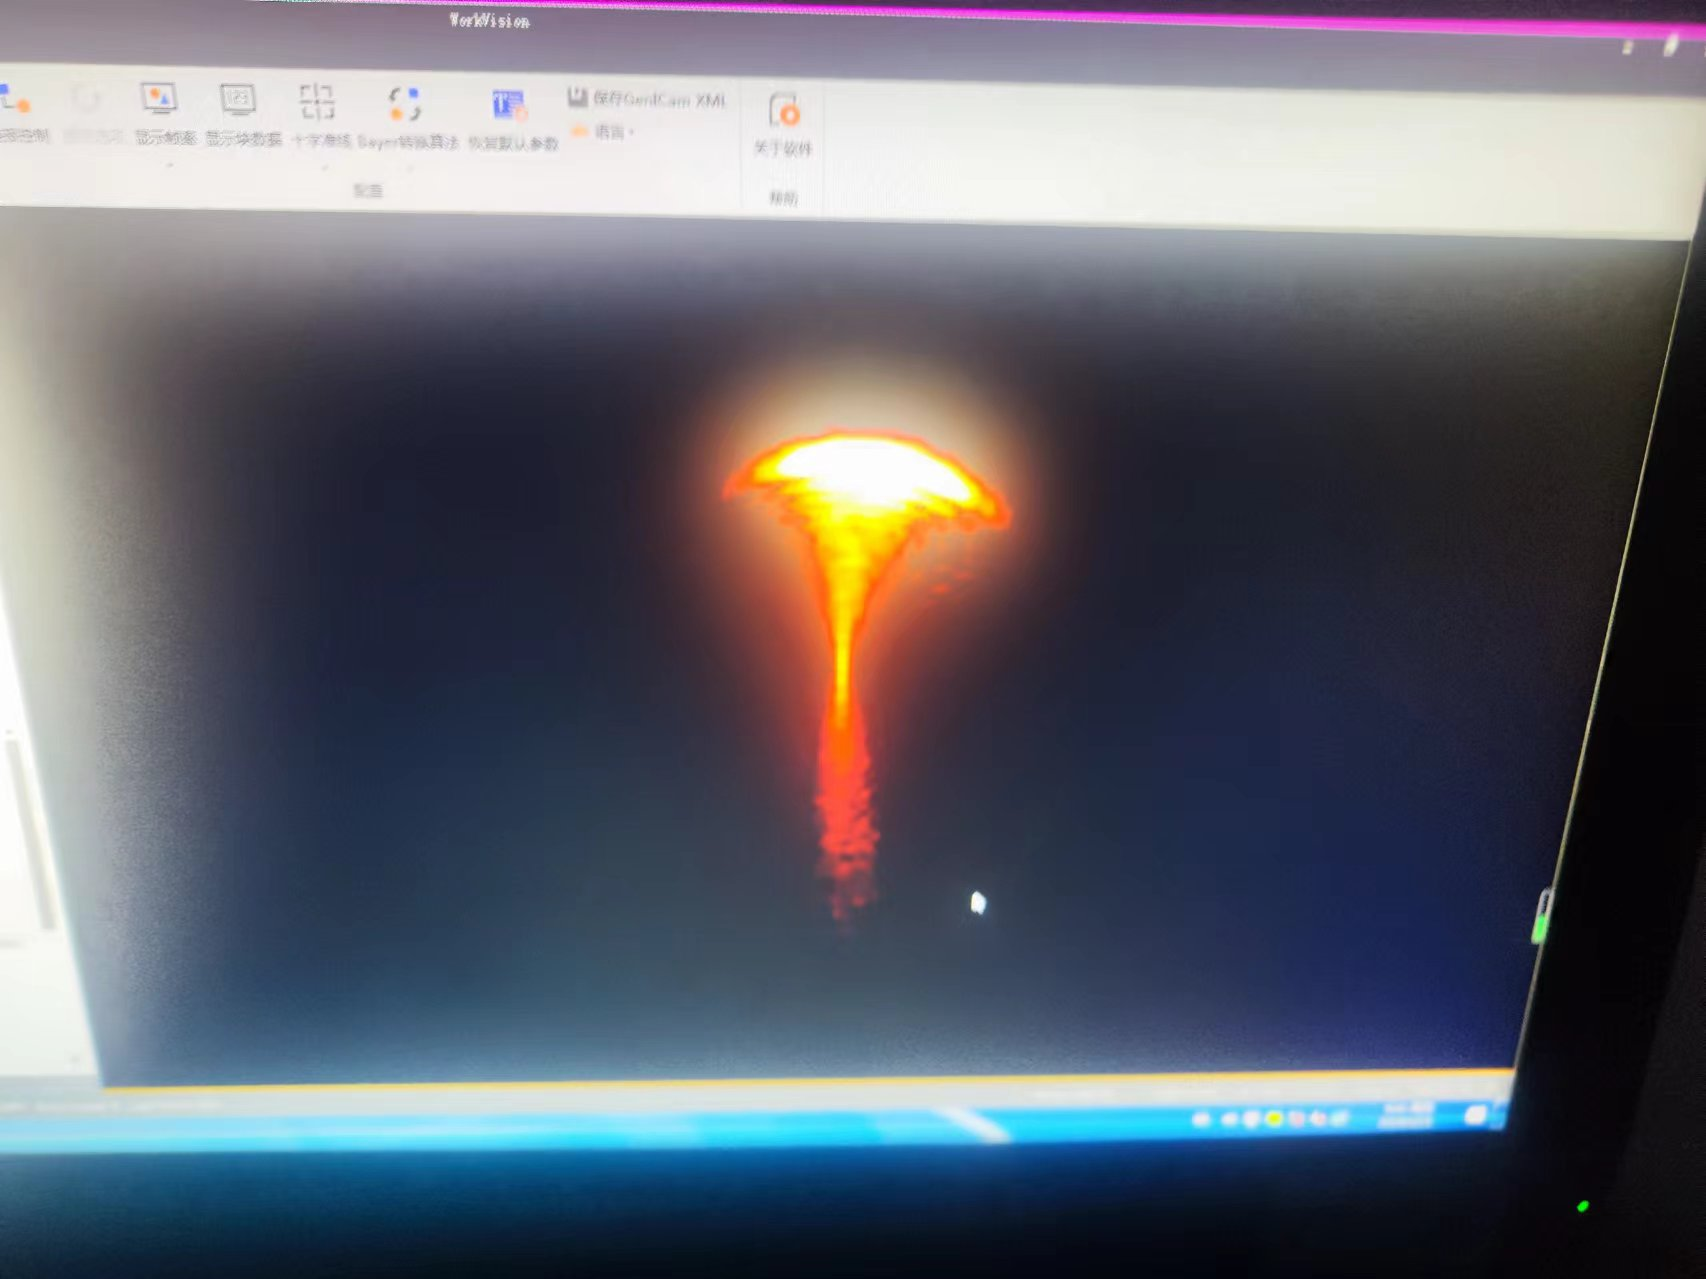
\includegraphics[width=0.35\linewidth]{错误.jpg}
		\caption{错误实验图像}
		\label{错误实验图像}
		\end{figure}
	

	
	\end{enumerate}
	
	
	
	% 分析与讨论	
	\clearpage
	
	% 顶栏
	\begin{table}
		\renewcommand\arraystretch{1.7}
		\begin{tabularx}{\textwidth}{|X|X|X|X|}
			\hline
			专业:& 物理学 &年级:& 2022级\\
			\hline
			姓名: &  黄罗琳& 学号:&22344001 \\
			\hline
			日期:& 2024/3/21 & 评分: &   \\
			\hline
		\end{tabularx}
	\end{table}
	% ---
	
	% 小标题
	\section{CD1 光学像差测量与分析\quad\heiti 分析与讨论}
	% ---
	
	% 数据处理
	\subsection{实验数据分析}
	
	%
	\subsubsection{}
	\begin{enumerate}
		\item 
	\end{enumerate}
	
	%
	\subsubsection{}
	\begin{enumerate}
		\item 
	\end{enumerate}
	
	%
	\subsubsection{}
	
	% ---
	
	% 实验后思考题
	\subsection{实验后思考题}
	
	%思考题1
	\begin{question}
		
	\end{question}
	
	% 思考题2
	\begin{question}
		
	\end{question}
	
	% 思考题3
	\begin{question}
		
	\end{question}
	
	% ---
	
	
	% 结语部分
	\clearpage
	
	% 小标题
	\section{ETX 实验名称××× \quad\heiti 结语}
	% ---
	
	% 总结、杂谈与致谢
	\subsection{实验心得和体会、意见建议等}
	\begin{enumerate}
		\item 实验要求很大的耐心,例如实验主光路的调整会存在高度的问题,需要进行一次又一次的调整,秉持着“就高又就低”的原则,既要保证有最低高度限制的设备能够进入光路,也要保证最高有效调整高度的仪器能够稳定调节高低(五维调整机构),所以也要在试验一次次探索中了解到实验仪器的合适的高度区间。
		\item 对于实验总体效果,我发现了在实验一中,我在调整色差时会出现灯丝的像很亮从而无法分辨哪一个位置是最清晰的,我们可以同 
	\end{enumerate}
	% ---
	

	% 附件
	\subsection{附件及实验相关的软硬件资料等}
	试验台桌面整理如%\cref{}所示。
	
	实验报告个人签名如

	% ---
	
	
\end{document}